\documentclass{article}
\usepackage{graphicx} 
\usepackage[utf8]{inputenc}
\usepackage[a4paper, left=3cm, right=3cm, top=3.5cm, bottom=3.5cm, headsep=1.2cm]{geometry}
\usepackage{latexsym}
\usepackage[polish]{babel}

\title{\huge Akademia Górniczo-Hutnicza \\ im. Stanisława Staszica w Krakowie \\ \Large WEAIiIB}
\author{\huge Analiza Strukturalna Systemu \\ \huge Stoku Narciarskiego \\ \\ \\ \LARGE Przedmiot: Inżynieria Oprogramowania \\ \Large Autorzy: Piotr Kucharski, Dominik Zabłotny \\ Informatyka, rok III}

\date{2018/2019}

\begin{document}

\begin{figure}
\centering

\includegraphics[width=3cm]{agh.png}
\label{fig: agh}
\end{figure}

\maketitle

%%%%%%%%%%%%%%%%%%%%%%%%%%%%%%%%%%%%%%%%%%%%%%%%%%%%%%%%%%%%
\newpage
\tableofcontents
\newpage
\section{Streszczenie}
\large{
Celem systemu jest zapewnienie pracownikom oraz klientom kompleskowej obsługi w zakresie sprzedaży karnetów wjazdowych na stacji narciarskiej oraz serwisu \\ i wypożyczenia sprzętu zimowego. W celu utrzymania najwyzszych standardów obsługi klientów przeprowadzane są ankiety zadowolenia. \\ \\ Klient za pomocą systemu internetowego lub poprzez zakup w okienku sprzedaży może nabyć wybrane przez siebie karnety wjazdowe - punktowe lub czasowe. Przy zakupie klient określa typ karnetu z puli dostępnych opcji sprzedaży tj. punktowy lub czasowy określony biznesowo. Klient ma do wyboru płatność gotówką, kartą lub przelewem. Po zaksięgowaniu wpłaty klient otrzymuje wybrany przez siebie karnet oraz potwierdzenie transakcji w postaci rachunku lub faktury. W przypadku kupna karnetu drogą elektroniczną karnet zostaje przypisany do osobistego karnetu lub \\ w przypadku zakupu w punkcie sprzedaży na nośnik magnetyczny jednorazowy. Jeżeli klient korzysta z osobistego nośnika karnetu zarejestrowanego w systemie, zostaje uprawniony do skorzystania ze zniżki 10\% przy zakupie karnetu czasowego. \\ \\ W systemie elektronicznym oraz w punkcie wypożyczeń istnieje możliwość \\ wypożyczenia sprzętu zimowego oraz serwisu własnych akcesoriów. Klient określa szczegóły takie jak czas wypożyczenia, rodzaj serwisu, ilość pobranego sprzętu. \\ \\ Losowo wybrani klienci zostają poproszeni o wypełnienie ankiety zadowolenia \\ z jakości świadczonych usług. Wyniki z ankiet zostają przekazane do systemu oraz są dostępne do analizy przez analityków stacji narciarskiej.}

\newpage

%%%%%%%%%%%%%%%%%%%%%%%%%%%%%%%%%%%%%%%%%%%%%%%%%%%%%%%%%%%%
\section{Sygnały zewnętrzne}
\begin{enumerate}
\item Wypełnienie formularza zakupu karnetu
\item Wypełnienie formularza wypożyczenia sprzętu
\item Wypełnienie formularza serwisu sprzętu
\item Złożenie zamówienia
\item Przyjęcie zamówienia do systemu
\item Wybór potwierdzenia zakupu
\item Wybór metody płatności
\item Zaksięgowanie płatności
\item Rozpoczęcie czasu świadczenia usługi
\item Zakończenie czasu świadczenia usługi
\item Realizacja serwisu
\item Przeprowadzenie ankiety satysfakcji
\end{enumerate}

%%%%%%%%%%%%%%%%%%%%%%%%%%%%%%%%%%%%%%%%%%%%%%%%%%%%%%%%%%%%
\newpage
\section{Diagram kontekstowy}

\begin{figure}[h]
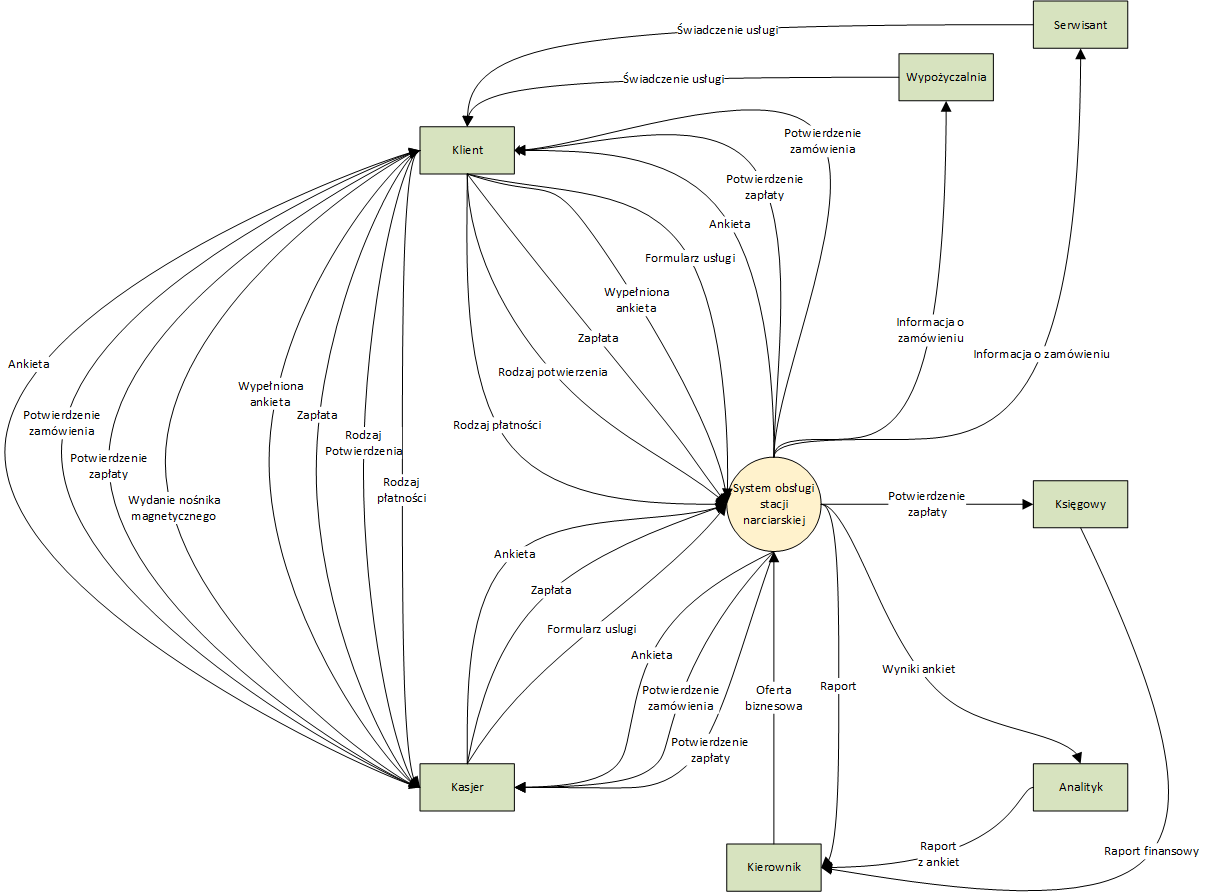
\includegraphics[scale=0.65]{diagram_kontekstowy.png}
\label{fig: diagram kontekstowy}
\end{figure}

%%%%%%%%%%%%%%%%%%%%%%%%%%%%%%%%%%%%%%%%%%%%%%%%%%%%%%%%%%%%
\newpage
\section{Model logiczny systemu}
\subsection{Diagram DFD - poziom 0}

\begin{figure}[h]
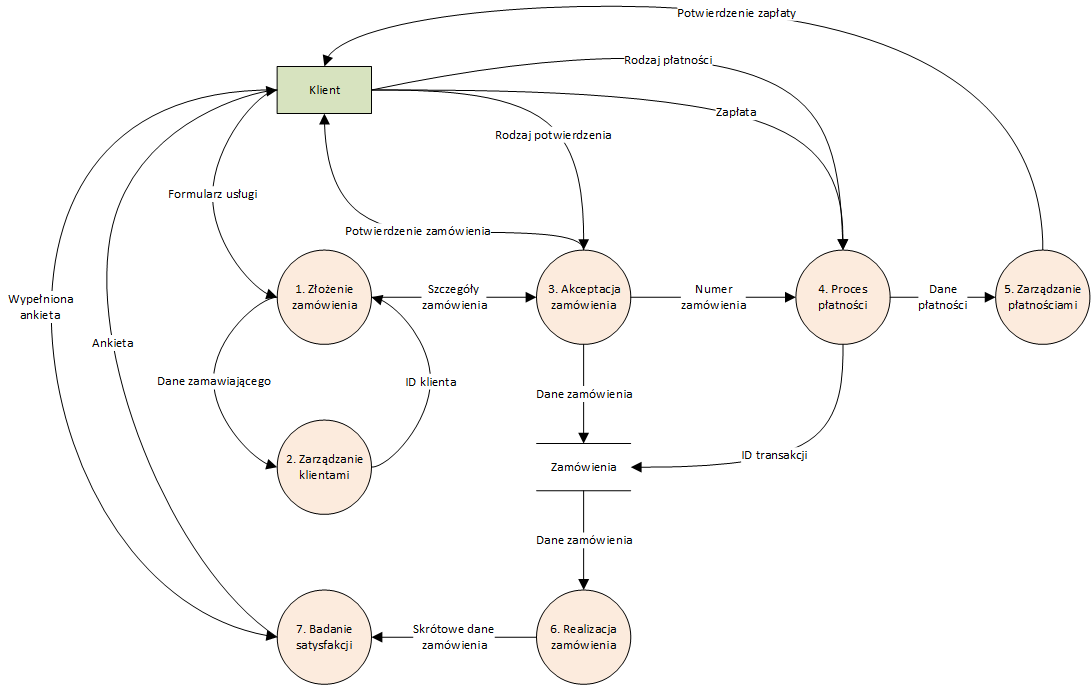
\includegraphics[scale=0.7]{dfd.png}
\label{fig: dfd0}
\end{figure}




\end{document}
